% Generado por demo/deck/build.py (HACK-088). No editar: cambiar build.py y reconstruir.
\documentclass[t]{beamer}
\geometry{papersize={720bp,405bp}}
\setbeamertemplate{navigation symbols}{}
\hypersetup{pdftitle={Stuff+ 2240 · Diablos Rojos · deck v2}}
\usepackage[sfdefault,lining]{FiraSans}
\usepackage{graphicx}
\usepackage{tikz}
\setlength{\parindent}{0pt}
\begin{document}

\begin{frame}[plain]
\begin{tikzpicture}[remember picture, overlay, x=1bp, y=1bp, shift={(current page.south west)}]
\fill[color={rgb,255:red,18;green,19;blue,22}] (0.00,405.00) rectangle (720.00,0.00);
\fill[color={rgb,255:red,215;green,25;blue,32}] (0.00,405.00) rectangle (6.00,0.00);
\fill[color={rgb,255:red,215;green,25;blue,32}] (40.00,381.00) rectangle (48.00,373.00);
\node[anchor=base west, inner sep=0, text={rgb,255:red,158;green,161;blue,167}, font=\fontsize{9bp}{10.8bp}\selectfont\bfseries] at (56.00,376.62) {STUFF+ 2240 / DIABLOS ROJOS};
\node[anchor=base west, inner sep=0, text={rgb,255:red,215;green,25;blue,32}, font=\fontsize{11bp}{13.2bp}\selectfont\bfseries] at (656.00,374.98) {01};
\node[anchor=base west, inner sep=0, text={rgb,255:red,244;green,244;blue,245}, font=\fontsize{25bp}{30.0bp}\selectfont\bfseries] at (40.00,336.50) {El mismo arsenal pierde 13.0 puntos};
\node[anchor=base west, inner sep=0, text={rgb,255:red,244;green,244;blue,245}, font=\fontsize{25bp}{30.0bp}\selectfont\bfseries] at (40.00,306.50) {de Stuff+ en el aire de CDMX};
\fill[color={rgb,255:red,31;green,33;blue,37}] (40.00,45.00) rectangle (680.00,44.20);
\node[anchor=base west, inner sep=0, text={rgb,255:red,158;green,161;blue,167}, font=\fontsize{7.5bp}{9.0bp}\selectfont] at (40.00,29.85) {reports/altitude\_delta/delta\_by\_shape.csv · promedio de la liga = ΔStuff+ de una forma − su diferencia contra la liga.};
\node[anchor=base west, inner sep=0, text={rgb,255:red,215;green,25;blue,32}, font=\fontsize{84bp}{100.8bp}\selectfont\bfseries] at (40.00,208.12) {−13.0};
\node[anchor=base west, inner sep=0, text={rgb,255:red,244;green,244;blue,245}, font=\fontsize{14.5bp}{17.4bp}\selectfont\bfseries] at (345.00,253.11) {ΔStuff+ de la liga en el aire del Harp};
\node[anchor=base west, inner sep=0, text={rgb,255:red,244;green,244;blue,245}, font=\fontsize{14.5bp}{17.4bp}\selectfont\bfseries] at (345.00,233.11) {Helú.};
\node[anchor=base west, inner sep=0, text={rgb,255:red,158;green,161;blue,167}, font=\fontsize{14bp}{16.8bp}\selectfont] at (345.00,203.52) {El modelo mide el aire de cada juego y lo};
\node[anchor=base west, inner sep=0, text={rgb,255:red,158;green,161;blue,167}, font=\fontsize{14bp}{16.8bp}\selectfont] at (345.00,184.52) {extrapola a un aire que no vio.};
\fill[color={rgb,255:red,31;green,33;blue,37}, rounded corners=6bp] (40.00,143.00) rectangle (680.00,85.00);
\fill[color={rgb,255:red,215;green,25;blue,32}] (40.00,143.00) rectangle (44.00,85.00);
\node[anchor=base west, inner sep=0, text={rgb,255:red,244;green,244;blue,245}, font=\fontsize{13bp}{15.6bp}\selectfont] at (58.00,120.34) {Datos oficiales agregados. Identificación inferida: la sede del staff};
\node[anchor=base west, inner sep=0, text={rgb,255:red,244;green,244;blue,245}, font=\fontsize{13bp}{15.6bp}\selectfont] at (58.00,102.34) {sigue sin confirmarse.};
\end{tikzpicture}
\end{frame}
\begin{frame}[plain]
\begin{tikzpicture}[remember picture, overlay, x=1bp, y=1bp, shift={(current page.south west)}]
\fill[color={rgb,255:red,18;green,19;blue,22}] (0.00,405.00) rectangle (720.00,0.00);
\fill[color={rgb,255:red,215;green,25;blue,32}] (0.00,405.00) rectangle (6.00,0.00);
\fill[color={rgb,255:red,215;green,25;blue,32}] (40.00,381.00) rectangle (48.00,373.00);
\node[anchor=base west, inner sep=0, text={rgb,255:red,158;green,161;blue,167}, font=\fontsize{9bp}{10.8bp}\selectfont\bfseries] at (56.00,376.62) {STUFF+ 2240 / DIABLOS ROJOS};
\node[anchor=base west, inner sep=0, text={rgb,255:red,215;green,25;blue,32}, font=\fontsize{11bp}{13.2bp}\selectfont\bfseries] at (656.00,374.98) {02};
\node[anchor=base west, inner sep=0, text={rgb,255:red,244;green,244;blue,245}, font=\fontsize{25bp}{30.0bp}\selectfont\bfseries] at (40.00,336.50) {El aire estimado cambia entre ambientes};
\fill[color={rgb,255:red,31;green,33;blue,37}] (40.00,45.00) rectangle (680.00,44.20);
\node[anchor=base west, inner sep=0, text={rgb,255:red,158;green,161;blue,167}, font=\fontsize{7.5bp}{9.0bp}\selectfont] at (40.00,29.85) {reports/physics/rho\_by\_bucket.csv · media por bucket; parques anónimos.};
\node[anchor=base west, inner sep=0, text={rgb,255:red,244;green,244;blue,245}, font=\fontsize{14bp}{16.8bp}\selectfont] at (40.00,253.52) {Nivel del mar};
\fill[color={rgb,255:red,31;green,33;blue,37}, rounded corners=3bp] (215.00,265.00) rectangle (550.00,247.00);
\fill[color={rgb,255:red,158;green,161;blue,167}, rounded corners=3bp] (215.00,265.00) rectangle (519.85,247.00);
\node[anchor=base west, inner sep=0, text={rgb,255:red,244;green,244;blue,245}, font=\fontsize{16bp}{19.2bp}\selectfont\bfseries] at (564.00,251.88) {1.001};
\node[anchor=base west, inner sep=0, text={rgb,255:red,244;green,244;blue,245}, font=\fontsize{14bp}{16.8bp}\selectfont] at (40.00,197.52) {Altitud media};
\fill[color={rgb,255:red,31;green,33;blue,37}, rounded corners=3bp] (215.00,209.00) rectangle (550.00,191.00);
\fill[color={rgb,255:red,158;green,161;blue,167}, rounded corners=3bp] (215.00,209.00) rectangle (486.65,191.00);
\node[anchor=base west, inner sep=0, text={rgb,255:red,244;green,244;blue,245}, font=\fontsize{16bp}{19.2bp}\selectfont\bfseries] at (564.00,195.88) {0.892};
\node[anchor=base west, inner sep=0, text={rgb,255:red,244;green,244;blue,245}, font=\fontsize{14bp}{16.8bp}\selectfont] at (40.00,141.52) {Altitud extrema};
\fill[color={rgb,255:red,31;green,33;blue,37}, rounded corners=3bp] (215.00,153.00) rectangle (550.00,135.00);
\fill[color={rgb,255:red,215;green,25;blue,32}, rounded corners=3bp] (215.00,153.00) rectangle (471.12,135.00);
\node[anchor=base west, inner sep=0, text={rgb,255:red,244;green,244;blue,245}, font=\fontsize{16bp}{19.2bp}\selectfont\bfseries] at (564.00,139.88) {0.841};
\node[anchor=base west, inner sep=0, text={rgb,255:red,158;green,161;blue,167}, font=\fontsize{12bp}{14.4bp}\selectfont] at (40.00,89.16) {Densidad relativa: menor valor significa aire menos denso.};
\end{tikzpicture}
\end{frame}
\begin{frame}[plain]
\begin{tikzpicture}[remember picture, overlay, x=1bp, y=1bp, shift={(current page.south west)}]
\fill[color={rgb,255:red,18;green,19;blue,22}] (0.00,405.00) rectangle (720.00,0.00);
\fill[color={rgb,255:red,215;green,25;blue,32}] (0.00,405.00) rectangle (6.00,0.00);
\fill[color={rgb,255:red,215;green,25;blue,32}] (40.00,381.00) rectangle (48.00,373.00);
\node[anchor=base west, inner sep=0, text={rgb,255:red,158;green,161;blue,167}, font=\fontsize{9bp}{10.8bp}\selectfont\bfseries] at (56.00,376.62) {STUFF+ 2240 / DIABLOS ROJOS};
\node[anchor=base west, inner sep=0, text={rgb,255:red,215;green,25;blue,32}, font=\fontsize{11bp}{13.2bp}\selectfont\bfseries] at (656.00,374.98) {03};
\node[anchor=base west, inner sep=0, text={rgb,255:red,244;green,244;blue,245}, font=\fontsize{25bp}{30.0bp}\selectfont\bfseries] at (40.00,336.50) {La recta pierde subida: el Magnus cae};
\node[anchor=base west, inner sep=0, text={rgb,255:red,244;green,244;blue,245}, font=\fontsize{25bp}{30.0bp}\selectfont\bfseries] at (40.00,306.50) {más rápido que el aire};
\fill[color={rgb,255:red,31;green,33;blue,37}] (40.00,45.00) rectangle (680.00,44.20);
\node[anchor=base west, inner sep=0, text={rgb,255:red,158;green,161;blue,167}, font=\fontsize{7.5bp}{9.0bp}\selectfont] at (40.00,29.85) {reports/physics/delta\_extreme\_vs\_no.csv; reports/altitude\_delta/delta\_by\_shape.csv · 4S; reports/physics\_v2/magnus\_elasticity.csv.};
\fill[color={rgb,255:red,31;green,33;blue,37}, rounded corners=6bp] (40.00,283.00) rectangle (236.00,117.00);
\node[anchor=base west, inner sep=0, text={rgb,255:red,215;green,25;blue,32}, font=\fontsize{40bp}{48.0bp}\selectfont\bfseries] at (56.00,234.20) {−3.54"};
\node[anchor=base west, inner sep=0, text={rgb,255:red,244;green,244;blue,245}, font=\fontsize{13bp}{15.6bp}\selectfont] at (56.00,202.34) {Observado};
\node[anchor=base west, inner sep=0, text={rgb,255:red,244;green,244;blue,245}, font=\fontsize{13bp}{15.6bp}\selectfont] at (56.00,185.44) {altitud extrema − sin};
\node[anchor=base west, inner sep=0, text={rgb,255:red,244;green,244;blue,245}, font=\fontsize{13bp}{15.6bp}\selectfont] at (56.00,168.54) {altitud};
\fill[color={rgb,255:red,31;green,33;blue,37}, rounded corners=6bp] (262.00,283.00) rectangle (458.00,117.00);
\node[anchor=base west, inner sep=0, text={rgb,255:red,215;green,25;blue,32}, font=\fontsize{40bp}{48.0bp}\selectfont\bfseries] at (278.00,234.20) {−3.56"};
\node[anchor=base west, inner sep=0, text={rgb,255:red,244;green,244;blue,245}, font=\fontsize{13bp}{15.6bp}\selectfont] at (278.00,202.34) {Modelo, forma 4S};
\node[anchor=base west, inner sep=0, text={rgb,255:red,244;green,244;blue,245}, font=\fontsize{13bp}{15.6bp}\selectfont] at (278.00,185.44) {CDMX − nivel del mar};
\fill[color={rgb,255:red,31;green,33;blue,37}, rounded corners=6bp] (484.00,283.00) rectangle (680.00,117.00);
\node[anchor=base west, inner sep=0, text={rgb,255:red,215;green,25;blue,32}, font=\fontsize{40bp}{48.0bp}\selectfont\bfseries] at (500.00,234.20) {1.36};
\node[anchor=base west, inner sep=0, text={rgb,255:red,244;green,244;blue,245}, font=\fontsize{13bp}{15.6bp}\selectfont] at (500.00,202.34) {Elasticidad del Magnus};
\node[anchor=base west, inner sep=0, text={rgb,255:red,244;green,244;blue,245}, font=\fontsize{13bp}{15.6bp}\selectfont] at (500.00,185.44) {de la recta (libro: 1)};
\node[anchor=base west, inner sep=0, text={rgb,255:red,158;green,161;blue,167}, font=\fontsize{12bp}{14.4bp}\selectfont] at (40.00,89.16) {IVB: movimiento vertical inducido, pulgadas. El simulador usa la elasticidad medida.};
\end{tikzpicture}
\end{frame}
\begin{frame}[plain]

\begin{tikzpicture}[remember picture, overlay, x=1bp, y=1bp, shift={(current page.south west)}]
\fill[color={rgb,255:red,18;green,19;blue,22}] (0.00,405.00) rectangle (720.00,0.00);
\fill[color={rgb,255:red,215;green,25;blue,32}] (0.00,405.00) rectangle (6.00,0.00);
\fill[color={rgb,255:red,215;green,25;blue,32}] (40.00,381.00) rectangle (48.00,373.00);
\node[anchor=base west, inner sep=0, text={rgb,255:red,158;green,161;blue,167}, font=\fontsize{9bp}{10.8bp}\selectfont\bfseries] at (56.00,376.62) {STUFF+ 2240 / DIABLOS ROJOS};
\node[anchor=base west, inner sep=0, text={rgb,255:red,215;green,25;blue,32}, font=\fontsize{11bp}{13.2bp}\selectfont\bfseries] at (656.00,374.98) {04};
\node[anchor=base west, inner sep=0, text={rgb,255:red,244;green,244;blue,245}, font=\fontsize{25bp}{30.0bp}\selectfont\bfseries] at (40.00,336.50) {Le ganamos al modelo nulo de la rúbrica};
\fill[color={rgb,255:red,31;green,33;blue,37}] (40.00,45.00) rectangle (680.00,44.20);
\node[anchor=base west, inner sep=0, text={rgb,255:red,158;green,161;blue,167}, font=\fontsize{7.5bp}{9.0bp}\selectfont] at (40.00,29.85) {reports/validation/headline.csv; reports/stuff\_v2/skill.csv; reports/stuff\_v2/pitcher\_level.csv.};
\node[anchor=base west, inner sep=0, text={rgb,255:red,244;green,244;blue,245}, font=\fontsize{14bp}{16.8bp}\selectfont] at (40.00,273.52) {Pitching+};
\fill[color={rgb,255:red,31;green,33;blue,37}, rounded corners=3bp] (215.00,285.00) rectangle (550.00,267.00);
\fill[color={rgb,255:red,215;green,25;blue,32}, rounded corners=3bp] (215.00,285.00) rectangle (474.96,267.00);
\node[anchor=base west, inner sep=0, text={rgb,255:red,244;green,244;blue,245}, font=\fontsize{16bp}{19.2bp}\selectfont\bfseries] at (564.00,271.88) {3.88 \%};
\node[anchor=base west, inner sep=0, text={rgb,255:red,244;green,244;blue,245}, font=\fontsize{14bp}{16.8bp}\selectfont] at (40.00,241.52) {Stuff+ v2};
\fill[color={rgb,255:red,31;green,33;blue,37}, rounded corners=3bp] (215.00,253.00) rectangle (550.00,235.00);
\fill[color={rgb,255:red,215;green,25;blue,32}, rounded corners=3bp] (215.00,253.00) rectangle (227.06,235.00);
\node[anchor=base west, inner sep=0, text={rgb,255:red,244;green,244;blue,245}, font=\fontsize{16bp}{19.2bp}\selectfont\bfseries] at (564.00,239.88) {+0.18 \%};
\node[anchor=base west, inner sep=0, text={rgb,255:red,158;green,161;blue,167}, font=\fontsize{11bp}{13.2bp}\selectfont] at (40.00,211.98) {\% de RMSE que baja frente al nulo por conteo, validación por pitcher.};
\fill[color={rgb,255:red,31;green,33;blue,37}, rounded corners=6bp] (40.00,195.00) rectangle (356.00,75.00);
\node[anchor=base west, inner sep=0, text={rgb,255:red,215;green,25;blue,32}, font=\fontsize{34bp}{40.8bp}\selectfont\bfseries] at (56.00,151.12) {0.269};
\node[anchor=base west, inner sep=0, text={rgb,255:red,244;green,244;blue,245}, font=\fontsize{12bp}{14.4bp}\selectfont] at (56.00,122.06) {r de Stuff+ v2 con 50 lanzamientos contra};
\node[anchor=base west, inner sep=0, text={rgb,255:red,244;green,244;blue,245}, font=\fontsize{12bp}{14.4bp}\selectfont] at (56.00,106.46) {el resto de la temporada};
\fill[color={rgb,255:red,31;green,33;blue,37}, rounded corners=6bp] (364.00,195.00) rectangle (680.00,75.00);
\node[anchor=base west, inner sep=0, text={rgb,255:red,158;green,161;blue,167}, font=\fontsize{34bp}{40.8bp}\selectfont\bfseries] at (380.00,151.12) {0.048};
\node[anchor=base west, inner sep=0, text={rgb,255:red,244;green,244;blue,245}, font=\fontsize{12bp}{14.4bp}\selectfont] at (380.00,122.06) {r de los resultados del propio pitcher};
\node[anchor=base west, inner sep=0, text={rgb,255:red,244;green,244;blue,245}, font=\fontsize{12bp}{14.4bp}\selectfont] at (380.00,106.46) {con los mismos 50 lanzamientos};
\end{tikzpicture}
\end{frame}
\begin{frame}[plain]
\begin{tikzpicture}[remember picture, overlay, x=1bp, y=1bp, shift={(current page.south west)}]
\fill[color={rgb,255:red,18;green,19;blue,22}] (0.00,405.00) rectangle (720.00,0.00);
\fill[color={rgb,255:red,215;green,25;blue,32}] (0.00,405.00) rectangle (6.00,0.00);
\fill[color={rgb,255:red,215;green,25;blue,32}] (40.00,381.00) rectangle (48.00,373.00);
\node[anchor=base west, inner sep=0, text={rgb,255:red,158;green,161;blue,167}, font=\fontsize{9bp}{10.8bp}\selectfont\bfseries] at (56.00,376.62) {STUFF+ 2240 / DIABLOS ROJOS};
\node[anchor=base west, inner sep=0, text={rgb,255:red,215;green,25;blue,32}, font=\fontsize{11bp}{13.2bp}\selectfont\bfseries] at (656.00,374.98) {05};
\node[anchor=base west, inner sep=0, text={rgb,255:red,244;green,244;blue,245}, font=\fontsize{25bp}{30.0bp}\selectfont\bfseries] at (40.00,336.50) {La física corrige el sesgo de altitud};
\fill[color={rgb,255:red,31;green,33;blue,37}] (40.00,45.00) rectangle (680.00,44.20);
\node[anchor=base west, inner sep=0, text={rgb,255:red,158;green,161;blue,167}, font=\fontsize{7.5bp}{9.0bp}\selectfont] at (40.00,29.85) {reports/stuff\_v2/altitude\_bias.csv · entrenado sin altitud extrema, evaluado en ella.};
\node[anchor=base west, inner sep=0, text={rgb,255:red,244;green,244;blue,245}, font=\fontsize{14bp}{16.8bp}\selectfont] at (40.00,267.52) {Nulo (conteo)};
\fill[color={rgb,255:red,31;green,33;blue,37}, rounded corners=3bp] (215.00,279.00) rectangle (550.00,261.00);
\fill[color={rgb,255:red,158;green,161;blue,167}, rounded corners=3bp] (215.00,279.00) rectangle (516.50,261.00);
\node[anchor=base west, inner sep=0, text={rgb,255:red,244;green,244;blue,245}, font=\fontsize{16bp}{19.2bp}\selectfont\bfseries] at (564.00,265.88) {+0.0108};
\node[anchor=base west, inner sep=0, text={rgb,255:red,244;green,244;blue,245}, font=\fontsize{14bp}{16.8bp}\selectfont] at (40.00,229.52) {Stuff+ v1};
\fill[color={rgb,255:red,31;green,33;blue,37}, rounded corners=3bp] (215.00,241.00) rectangle (550.00,223.00);
\fill[color={rgb,255:red,215;green,25;blue,32}, rounded corners=3bp] (215.00,241.00) rectangle (284.79,223.00);
\node[anchor=base west, inner sep=0, text={rgb,255:red,244;green,244;blue,245}, font=\fontsize{16bp}{19.2bp}\selectfont\bfseries] at (564.00,227.88) {+0.0025};
\node[anchor=base west, inner sep=0, text={rgb,255:red,244;green,244;blue,245}, font=\fontsize{14bp}{16.8bp}\selectfont] at (40.00,191.52) {Stuff+ v2};
\fill[color={rgb,255:red,31;green,33;blue,37}, rounded corners=3bp] (215.00,203.00) rectangle (550.00,185.00);
\fill[color={rgb,255:red,215;green,25;blue,32}, rounded corners=3bp] (215.00,203.00) rectangle (265.25,185.00);
\node[anchor=base west, inner sep=0, text={rgb,255:red,244;green,244;blue,245}, font=\fontsize{16bp}{19.2bp}\selectfont\bfseries] at (564.00,189.88) {+0.0018};
\fill[color={rgb,255:red,31;green,33;blue,37}, rounded corners=6bp] (40.00,159.00) rectangle (680.00,115.00);
\fill[color={rgb,255:red,215;green,25;blue,32}] (40.00,159.00) rectangle (44.00,115.00);
\node[anchor=base west, inner sep=0, text={rgb,255:red,244;green,244;blue,245}, font=\fontsize{17bp}{20.4bp}\selectfont\bfseries] at (58.00,132.06) {Stuff+ v2 recorta el sesgo 84 \% frente al nulo.};
\node[anchor=base west, inner sep=0, text={rgb,255:red,158;green,161;blue,167}, font=\fontsize{12bp}{14.4bp}\selectfont] at (40.00,89.16) {Carreras por lanzamiento que el modelo subestima en un aire que no vio.};
\end{tikzpicture}
\end{frame}
\begin{frame}[plain]
\begin{tikzpicture}[remember picture, overlay, x=1bp, y=1bp, shift={(current page.south west)}]
\fill[color={rgb,255:red,18;green,19;blue,22}] (0.00,405.00) rectangle (720.00,0.00);
\fill[color={rgb,255:red,215;green,25;blue,32}] (0.00,405.00) rectangle (6.00,0.00);
\fill[color={rgb,255:red,215;green,25;blue,32}] (40.00,381.00) rectangle (48.00,373.00);
\node[anchor=base west, inner sep=0, text={rgb,255:red,158;green,161;blue,167}, font=\fontsize{9bp}{10.8bp}\selectfont\bfseries] at (56.00,376.62) {STUFF+ 2240 / DIABLOS ROJOS};
\node[anchor=base west, inner sep=0, text={rgb,255:red,215;green,25;blue,32}, font=\fontsize{11bp}{13.2bp}\selectfont\bfseries] at (656.00,374.98) {06};
\node[anchor=base west, inner sep=0, text={rgb,255:red,244;green,244;blue,245}, font=\fontsize{25bp}{30.0bp}\selectfont\bfseries] at (40.00,336.50) {Las pérdidas dependen de la forma del pitch};
\fill[color={rgb,255:red,31;green,33;blue,37}] (40.00,45.00) rectangle (680.00,44.20);
\node[anchor=base west, inner sep=0, text={rgb,255:red,158;green,161;blue,167}, font=\fontsize{7.5bp}{9.0bp}\selectfont] at (40.00,29.85) {reports/altitude\_delta/delta\_by\_shape.csv · delta\_stuff; misma forma, CDMX menos nivel del mar.};
\node[anchor=base west, inner sep=0, text={rgb,255:red,244;green,244;blue,245}, font=\fontsize{14bp}{16.8bp}\selectfont] at (40.00,271.52) {Curva 12-6};
\fill[color={rgb,255:red,31;green,33;blue,37}, rounded corners=3bp] (215.00,283.00) rectangle (550.00,265.00);
\fill[color={rgb,255:red,158;green,161;blue,167}, rounded corners=3bp] (215.00,283.00) rectangle (382.50,265.00);
\node[anchor=base west, inner sep=0, text={rgb,255:red,244;green,244;blue,245}, font=\fontsize{16bp}{19.2bp}\selectfont\bfseries] at (564.00,269.88) {−9.5};
\node[anchor=base west, inner sep=0, text={rgb,255:red,244;green,244;blue,245}, font=\fontsize{14bp}{16.8bp}\selectfont] at (40.00,233.52) {Sweeper};
\fill[color={rgb,255:red,31;green,33;blue,37}, rounded corners=3bp] (215.00,245.00) rectangle (550.00,227.00);
\fill[color={rgb,255:red,158;green,161;blue,167}, rounded corners=3bp] (215.00,245.00) rectangle (384.26,227.00);
\node[anchor=base west, inner sep=0, text={rgb,255:red,244;green,244;blue,245}, font=\fontsize{16bp}{19.2bp}\selectfont\bfseries] at (564.00,231.88) {−9.6};
\node[anchor=base west, inner sep=0, text={rgb,255:red,244;green,244;blue,245}, font=\fontsize{14bp}{16.8bp}\selectfont] at (40.00,195.52) {Recta 4S};
\fill[color={rgb,255:red,31;green,33;blue,37}, rounded corners=3bp] (215.00,207.00) rectangle (550.00,189.00);
\fill[color={rgb,255:red,158;green,161;blue,167}, rounded corners=3bp] (215.00,207.00) rectangle (416.00,189.00);
\node[anchor=base west, inner sep=0, text={rgb,255:red,244;green,244;blue,245}, font=\fontsize{16bp}{19.2bp}\selectfont\bfseries] at (564.00,193.88) {−11.4};
\node[anchor=base west, inner sep=0, text={rgb,255:red,244;green,244;blue,245}, font=\fontsize{14bp}{16.8bp}\selectfont] at (40.00,157.52) {Recta de ride};
\fill[color={rgb,255:red,31;green,33;blue,37}, rounded corners=3bp] (215.00,169.00) rectangle (550.00,151.00);
\fill[color={rgb,255:red,215;green,25;blue,32}, rounded corners=3bp] (215.00,169.00) rectangle (530.61,151.00);
\node[anchor=base west, inner sep=0, text={rgb,255:red,244;green,244;blue,245}, font=\fontsize{16bp}{19.2bp}\selectfont\bfseries] at (564.00,155.88) {−17.9};
\node[anchor=base west, inner sep=0, text={rgb,255:red,158;green,161;blue,167}, font=\fontsize{12bp}{14.4bp}\selectfont] at (40.00,89.16) {Longitud = pérdida de Stuff+. Ninguna forma gana en absoluto.};
\end{tikzpicture}
\end{frame}
\begin{frame}[plain]
\begin{tikzpicture}[remember picture, overlay, x=1bp, y=1bp, shift={(current page.south west)}]
\fill[color={rgb,255:red,18;green,19;blue,22}] (0.00,405.00) rectangle (720.00,0.00);
\fill[color={rgb,255:red,215;green,25;blue,32}] (0.00,405.00) rectangle (6.00,0.00);
\fill[color={rgb,255:red,215;green,25;blue,32}] (40.00,381.00) rectangle (48.00,373.00);
\node[anchor=base west, inner sep=0, text={rgb,255:red,158;green,161;blue,167}, font=\fontsize{9bp}{10.8bp}\selectfont\bfseries] at (56.00,376.62) {STUFF+ 2240 / DIABLOS ROJOS};
\node[anchor=base west, inner sep=0, text={rgb,255:red,215;green,25;blue,32}, font=\fontsize{11bp}{13.2bp}\selectfont\bfseries] at (656.00,374.98) {07};
\node[anchor=base west, inner sep=0, text={rgb,255:red,244;green,244;blue,245}, font=\fontsize{25bp}{30.0bp}\selectfont\bfseries] at (40.00,336.50) {Dos sedes candidatas, dos cuentas de};
\node[anchor=base west, inner sep=0, text={rgb,255:red,244;green,244;blue,245}, font=\fontsize{25bp}{30.0bp}\selectfont\bfseries] at (40.00,306.50) {carreras};
\fill[color={rgb,255:red,31;green,33;blue,37}] (40.00,45.00) rectangle (680.00,44.20);
\node[anchor=base west, inner sep=0, text={rgb,255:red,158;green,161;blue,167}, font=\fontsize{7.5bp}{9.0bp}\selectfont] at (40.00,29.85) {reports/staff\_audit/runs\_saved.csv · franquicias 5 y 11, por separado.};
\fill[color={rgb,255:red,31;green,33;blue,37}, rounded corners=6bp] (40.00,287.00) rectangle (356.00,129.00);
\node[anchor=base west, inner sep=0, text={rgb,255:red,158;green,161;blue,167}, font=\fontsize{14bp}{16.8bp}\selectfont\bfseries] at (58.00,261.52) {Franquicia 5};
\node[anchor=base west, inner sep=0, text={rgb,255:red,215;green,25;blue,32}, font=\fontsize{32bp}{38.4bp}\selectfont\bfseries] at (58.00,222.76) {6.5 carreras};
\node[anchor=base west, inner sep=0, text={rgb,255:red,244;green,244;blue,245}, font=\fontsize{15bp}{18.0bp}\selectfont] at (58.00,190.70) {0.46 victorias por temporada};
\node[anchor=base west, inner sep=0, text={rgb,255:red,158;green,161;blue,167}, font=\fontsize{13bp}{15.6bp}\selectfont] at (58.00,158.34) {Mezcla 5.2 · aperturas 1.4};
\fill[color={rgb,255:red,31;green,33;blue,37}, rounded corners=6bp] (364.00,287.00) rectangle (680.00,129.00);
\node[anchor=base west, inner sep=0, text={rgb,255:red,158;green,161;blue,167}, font=\fontsize{14bp}{16.8bp}\selectfont\bfseries] at (382.00,261.52) {Franquicia 11};
\node[anchor=base west, inner sep=0, text={rgb,255:red,215;green,25;blue,32}, font=\fontsize{32bp}{38.4bp}\selectfont\bfseries] at (382.00,222.76) {4.5 carreras};
\node[anchor=base west, inner sep=0, text={rgb,255:red,244;green,244;blue,245}, font=\fontsize{15bp}{18.0bp}\selectfont] at (382.00,190.70) {0.32 victorias por temporada};
\node[anchor=base west, inner sep=0, text={rgb,255:red,158;green,161;blue,167}, font=\fontsize{13bp}{15.6bp}\selectfont] at (382.00,158.34) {Mezcla 2.3 · aperturas 2.2};
\node[anchor=base west, inner sep=0, text={rgb,255:red,244;green,244;blue,245}, font=\fontsize{13bp}{15.6bp}\selectfont] at (40.00,104.34) {Identificación inferida. No se suman.};
\node[anchor=base west, inner sep=0, text={rgb,255:red,244;green,244;blue,245}, font=\fontsize{13bp}{15.6bp}\selectfont] at (40.00,87.34) {La sede sigue sin confirmarse.};
\end{tikzpicture}
\end{frame}
\begin{frame}[plain]
\begin{tikzpicture}[remember picture, overlay, x=1bp, y=1bp, shift={(current page.south west)}]
\fill[color={rgb,255:red,18;green,19;blue,22}] (0.00,405.00) rectangle (720.00,0.00);
\fill[color={rgb,255:red,215;green,25;blue,32}] (0.00,405.00) rectangle (6.00,0.00);
\fill[color={rgb,255:red,215;green,25;blue,32}] (40.00,381.00) rectangle (48.00,373.00);
\node[anchor=base west, inner sep=0, text={rgb,255:red,158;green,161;blue,167}, font=\fontsize{9bp}{10.8bp}\selectfont\bfseries] at (56.00,376.62) {STUFF+ 2240 / DIABLOS ROJOS};
\node[anchor=base west, inner sep=0, text={rgb,255:red,215;green,25;blue,32}, font=\fontsize{11bp}{13.2bp}\selectfont\bfseries] at (656.00,374.98) {08};
\node[anchor=base west, inner sep=0, text={rgb,255:red,244;green,244;blue,245}, font=\fontsize{25bp}{30.0bp}\selectfont\bfseries] at (40.00,336.50) {El producto: dos aires, un lanzamiento};
\fill[color={rgb,255:red,31;green,33;blue,37}] (40.00,45.00) rectangle (680.00,44.20);
\node[anchor=base west, inner sep=0, text={rgb,255:red,158;green,161;blue,167}, font=\fontsize{7.5bp}{9.0bp}\selectfont] at (40.00,29.85) {Capturas del simulador 3D y del explicador de física (Playwright, web/e2e/screenshots, HACK-051).};
\fill[color={rgb,255:red,31;green,33;blue,37}, rounded corners=4bp] (38.00,311.00) rectangle (350.00,129.00);
\node[anchor=north west, inner sep=0] at (40.00,309.00) {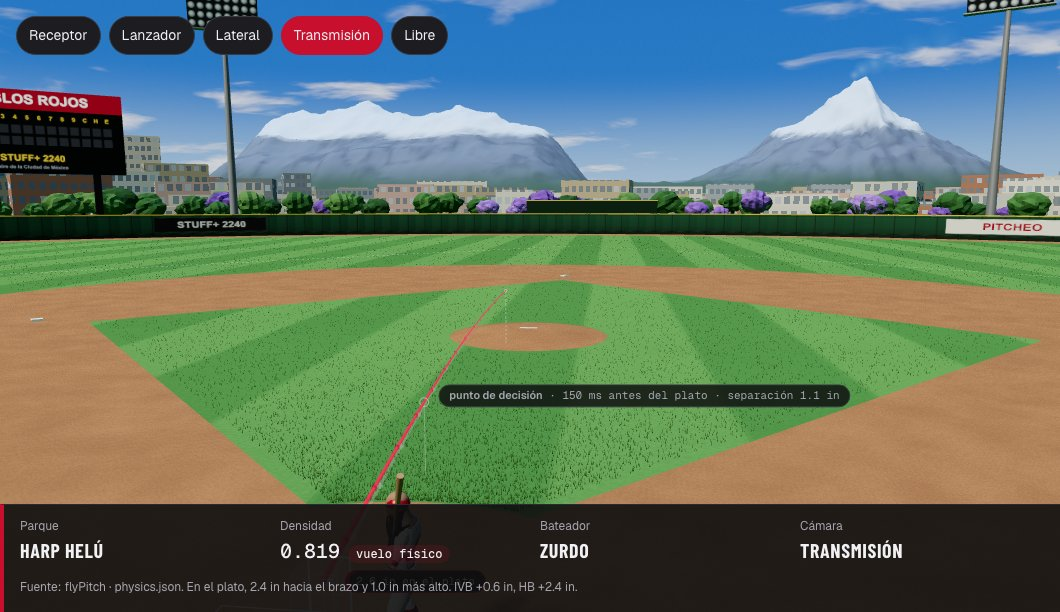
\includegraphics[width=308bp,height=178bp]{assets/simulador_transmision.jpg}};
\fill[color={rgb,255:red,31;green,33;blue,37}, rounded corners=4bp] (370.00,311.00) rectangle (682.00,109.00);
\node[anchor=north west, inner sep=0] at (372.00,309.00) {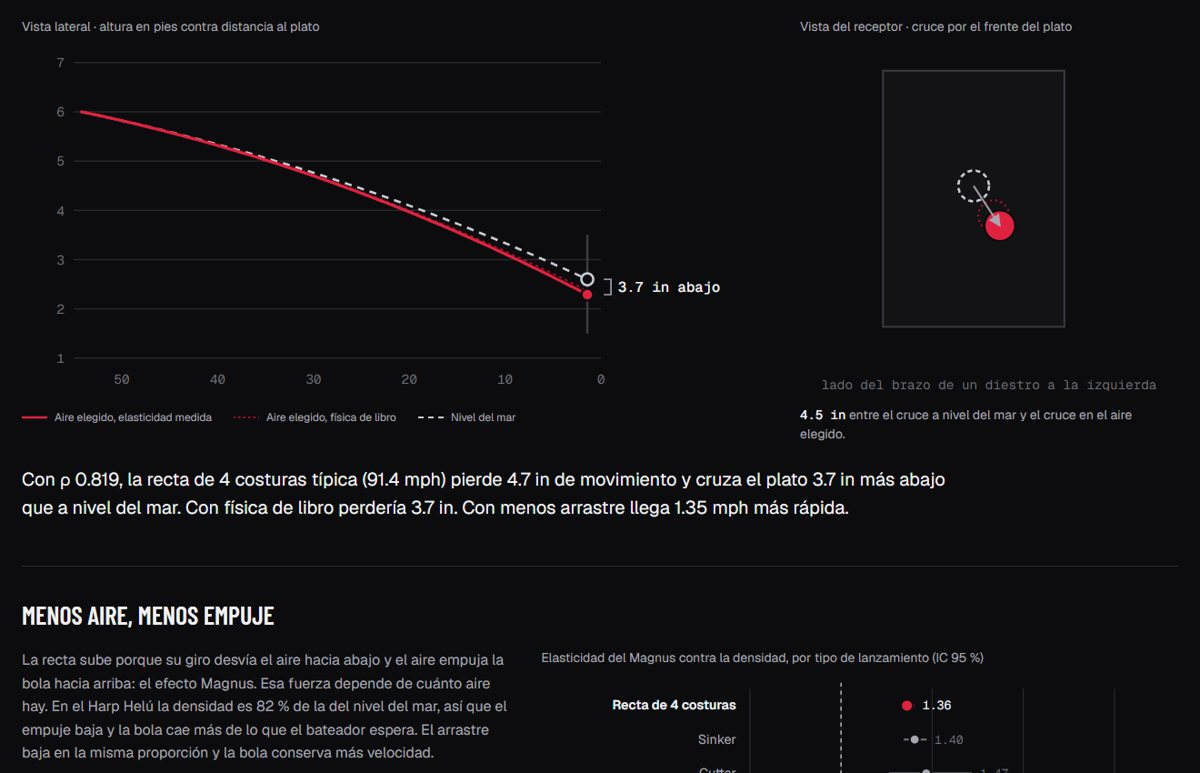
\includegraphics[width=308bp,height=198bp]{assets/fisica.jpg}};
\node[anchor=base west, inner sep=0, text={rgb,255:red,158;green,161;blue,167}, font=\fontsize{11bp}{13.2bp}\selectfont] at (40.00,109.98) {Simulador 3D: dos aires, mismo release.};
\node[anchor=base west, inner sep=0, text={rgb,255:red,158;green,161;blue,167}, font=\fontsize{11bp}{13.2bp}\selectfont] at (372.00,89.98) {Física: arrastre y Magnus contra la densidad.};
\end{tikzpicture}
\end{frame}
\begin{frame}[plain]
\begin{tikzpicture}[remember picture, overlay, x=1bp, y=1bp, shift={(current page.south west)}]
\fill[color={rgb,255:red,18;green,19;blue,22}] (0.00,405.00) rectangle (720.00,0.00);
\fill[color={rgb,255:red,215;green,25;blue,32}] (0.00,405.00) rectangle (6.00,0.00);
\fill[color={rgb,255:red,215;green,25;blue,32}] (40.00,381.00) rectangle (48.00,373.00);
\node[anchor=base west, inner sep=0, text={rgb,255:red,158;green,161;blue,167}, font=\fontsize{9bp}{10.8bp}\selectfont\bfseries] at (56.00,376.62) {STUFF+ 2240 / DIABLOS ROJOS};
\node[anchor=base west, inner sep=0, text={rgb,255:red,215;green,25;blue,32}, font=\fontsize{11bp}{13.2bp}\selectfont\bfseries] at (656.00,374.98) {09};
\node[anchor=base west, inner sep=0, text={rgb,255:red,244;green,244;blue,245}, font=\fontsize{25bp}{30.0bp}\selectfont\bfseries] at (40.00,336.50) {El entorno cambia el valor de una carrera};
\fill[color={rgb,255:red,31;green,33;blue,37}] (40.00,45.00) rectangle (680.00,44.20);
\node[anchor=base west, inner sep=0, text={rgb,255:red,158;green,161;blue,167}, font=\fontsize{7.5bp}{9.0bp}\selectfont] at (40.00,29.85) {reports/business\_value/runs\_per\_win.csv; reports/business\_value/gm\_example.csv · puntos de Stuff+ v2 fuera de pliegue.};
\fill[color={rgb,255:red,31;green,33;blue,37}, rounded corners=6bp] (40.00,287.00) rectangle (236.00,141.00);
\node[anchor=base west, inner sep=0, text={rgb,255:red,158;green,161;blue,167}, font=\fontsize{38bp}{45.6bp}\selectfont\bfseries] at (56.00,239.84) {11.8};
\node[anchor=base west, inner sep=0, text={rgb,255:red,244;green,244;blue,245}, font=\fontsize{13bp}{15.6bp}\selectfont] at (56.00,208.64) {Carreras por victoria};
\node[anchor=base west, inner sep=0, text={rgb,255:red,244;green,244;blue,245}, font=\fontsize{13bp}{15.6bp}\selectfont] at (56.00,191.74) {liga};
\fill[color={rgb,255:red,31;green,33;blue,37}, rounded corners=6bp] (262.00,287.00) rectangle (458.00,141.00);
\node[anchor=base west, inner sep=0, text={rgb,255:red,215;green,25;blue,32}, font=\fontsize{38bp}{45.6bp}\selectfont\bfseries] at (278.00,239.84) {14.3};
\node[anchor=base west, inner sep=0, text={rgb,255:red,244;green,244;blue,245}, font=\fontsize{13bp}{15.6bp}\selectfont] at (278.00,208.64) {Carreras por victoria};
\node[anchor=base west, inner sep=0, text={rgb,255:red,244;green,244;blue,245}, font=\fontsize{13bp}{15.6bp}\selectfont] at (278.00,191.74) {altitud extrema};
\fill[color={rgb,255:red,31;green,33;blue,37}, rounded corners=6bp] (484.00,287.00) rectangle (680.00,141.00);
\node[anchor=base west, inner sep=0, text={rgb,255:red,215;green,25;blue,32}, font=\fontsize{38bp}{45.6bp}\selectfont\bfseries] at (500.00,239.84) {1.51};
\node[anchor=base west, inner sep=0, text={rgb,255:red,244;green,244;blue,245}, font=\fontsize{13bp}{15.6bp}\selectfont] at (500.00,208.64) {Victorias en el Harp Helú};
\node[anchor=base west, inner sep=0, text={rgb,255:red,244;green,244;blue,245}, font=\fontsize{13bp}{15.6bp}\selectfont] at (500.00,191.74) {por +10 de Stuff+};
\node[anchor=base west, inner sep=0, text={rgb,255:red,244;green,244;blue,245}, font=\fontsize{15bp}{18.0bp}\selectfont\bfseries] at (40.00,112.70) {+10 puntos en 2,500 lanzamientos = 21.7 carreras (escenario).};
\node[anchor=base west, inner sep=0, text={rgb,255:red,158;green,161;blue,167}, font=\fontsize{12bp}{14.4bp}\selectfont] at (40.00,89.16) {El ahorro del staff está en la lámina 7, por franquicia.};
\end{tikzpicture}
\end{frame}
\begin{frame}[plain]
\begin{tikzpicture}[remember picture, overlay, x=1bp, y=1bp, shift={(current page.south west)}]
\fill[color={rgb,255:red,18;green,19;blue,22}] (0.00,405.00) rectangle (720.00,0.00);
\fill[color={rgb,255:red,215;green,25;blue,32}] (0.00,405.00) rectangle (6.00,0.00);
\fill[color={rgb,255:red,215;green,25;blue,32}] (40.00,381.00) rectangle (48.00,373.00);
\node[anchor=base west, inner sep=0, text={rgb,255:red,158;green,161;blue,167}, font=\fontsize{9bp}{10.8bp}\selectfont\bfseries] at (56.00,376.62) {STUFF+ 2240 / DIABLOS ROJOS};
\node[anchor=base west, inner sep=0, text={rgb,255:red,215;green,25;blue,32}, font=\fontsize{11bp}{13.2bp}\selectfont\bfseries] at (656.00,374.98) {10};
\node[anchor=base west, inner sep=0, text={rgb,255:red,244;green,244;blue,245}, font=\fontsize{25bp}{30.0bp}\selectfont\bfseries] at (40.00,336.50) {La demo compara el mismo arsenal};
\fill[color={rgb,255:red,31;green,33;blue,37}] (40.00,45.00) rectangle (680.00,44.20);
\node[anchor=base west, inner sep=0, text={rgb,255:red,158;green,161;blue,167}, font=\fontsize{7.5bp}{9.0bp}\selectfont] at (40.00,29.85) {Producto web en el repo. Respaldo: este PDF y los CSV agregados de reports/.};
\fill[color={rgb,255:red,31;green,33;blue,37}, rounded corners=4bp] (378.00,311.00) rectangle (682.00,134.00);
\node[anchor=north west, inner sep=0] at (380.00,309.00) {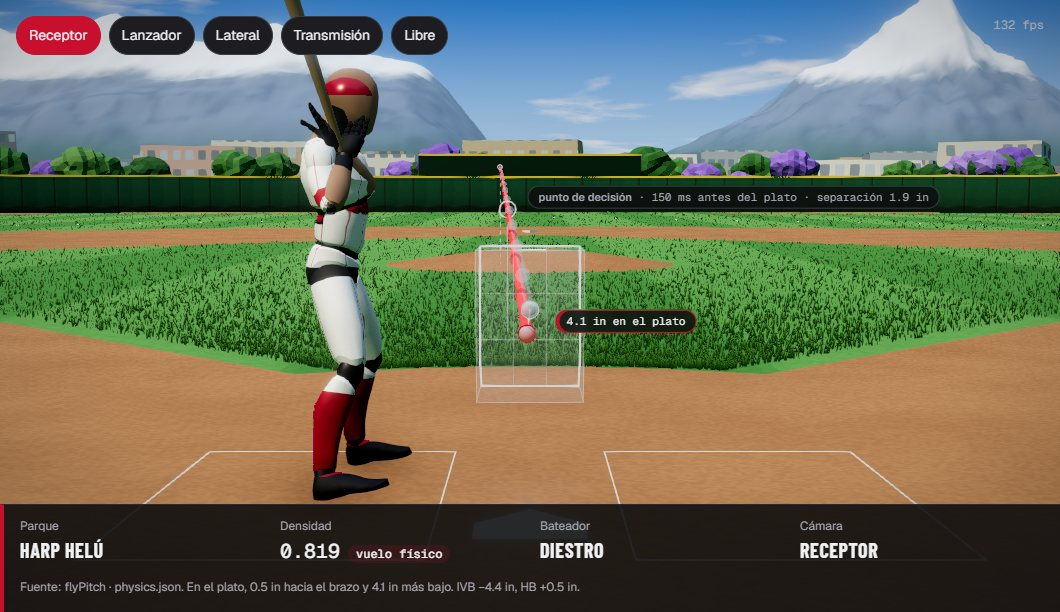
\includegraphics[width=300bp,height=173bp]{assets/simulador_receptor.jpg}};
\fill[color={rgb,255:red,215;green,25;blue,32}] (40.00,301.00) rectangle (44.00,265.00);
\node[anchor=base west, inner sep=0, text={rgb,255:red,244;green,244;blue,245}, font=\fontsize{15bp}{18.0bp}\selectfont\bfseries] at (56.00,282.70) {Simulador: la misma forma, dos};
\node[anchor=base west, inner sep=0, text={rgb,255:red,244;green,244;blue,245}, font=\fontsize{15bp}{18.0bp}\selectfont\bfseries] at (56.00,264.10) {aires.};
\fill[color={rgb,255:red,215;green,25;blue,32}] (40.00,249.00) rectangle (44.00,213.00);
\node[anchor=base west, inner sep=0, text={rgb,255:red,244;green,244;blue,245}, font=\fontsize{15bp}{18.0bp}\selectfont\bfseries] at (56.00,230.70) {Física: la densidad en vivo.};
\fill[color={rgb,255:red,215;green,25;blue,32}] (40.00,197.00) rectangle (44.00,161.00);
\node[anchor=base west, inner sep=0, text={rgb,255:red,244;green,244;blue,245}, font=\fontsize{15bp}{18.0bp}\selectfont\bfseries] at (56.00,178.70) {Altitud: los 20 parques por densidad.};
\node[anchor=base west, inner sep=0, text={rgb,255:red,158;green,161;blue,167}, font=\fontsize{13bp}{15.6bp}\selectfont] at (40.00,106.34) {Respaldo offline: este PDF y los CSV agregados.};
\node[anchor=base west, inner sep=0, text={rgb,255:red,158;green,161;blue,167}, font=\fontsize{13bp}{15.6bp}\selectfont] at (40.00,89.34) {La sede del staff sigue sin confirmarse.};
\end{tikzpicture}
\end{frame}
\end{document}
